\section{Modelos}

\subsection{Comparación del árbol baseline y ajustado}

El modelo \textbf{baseline}, entrenado con los parámetros por defecto, sirvió como referencia para validar el flujo de datos, el preprocesamiento y la capacidad del árbol para capturar patrones básicos en el conjunto \texttt{recidivism.csv}. En validación, el baseline alcanzó una \textbf{Accuracy (valid) = 0.659}, mostrando una estructura más profunda y fragmentada, con ramas menos coherentes entre sí y una ligera tendencia al sobreajuste. Aun así, permitió comprobar que las variables más relevantes —principalmente el número de antecedentes y la situación laboral— aparecían de forma recurrente en las divisiones iniciales, lo que validó el correcto preprocesamiento de los datos.

Tras aplicar \texttt{GridSearchCV} con validación estratificada de 5 pliegues, el árbol \textbf{ajustado} (\emph{tuned}) logró un mejor compromiso entre profundidad, precisión y legibilidad. El modelo redujo su complejidad a aproximadamente tres niveles y mejoró la consistencia de las reglas, alcanzando una \textbf{Accuracy (test) $\approx$ 0.70} y una \textbf{5-fold CV accuracy $\approx$ 0.719}. Las divisiones principales se concentraron en las variables \texttt{priors\_count}, \texttt{employment\_unemployed} y \texttt{age}, reflejando una jerarquía de decisión más lógica y estable.

En conjunto, el modelo ajustado mantiene la claridad visual del baseline, pero con reglas más compactas, generalización superior y un comportamiento más equilibrado entre clases, lo que confirma que un control adecuado de hiperparámetros puede mejorar simultáneamente la interpretabilidad y el rendimiento.

\begin{figure}[h]
  \centering
  \begin{subfigure}[t]{0.48\linewidth}
    \centering
    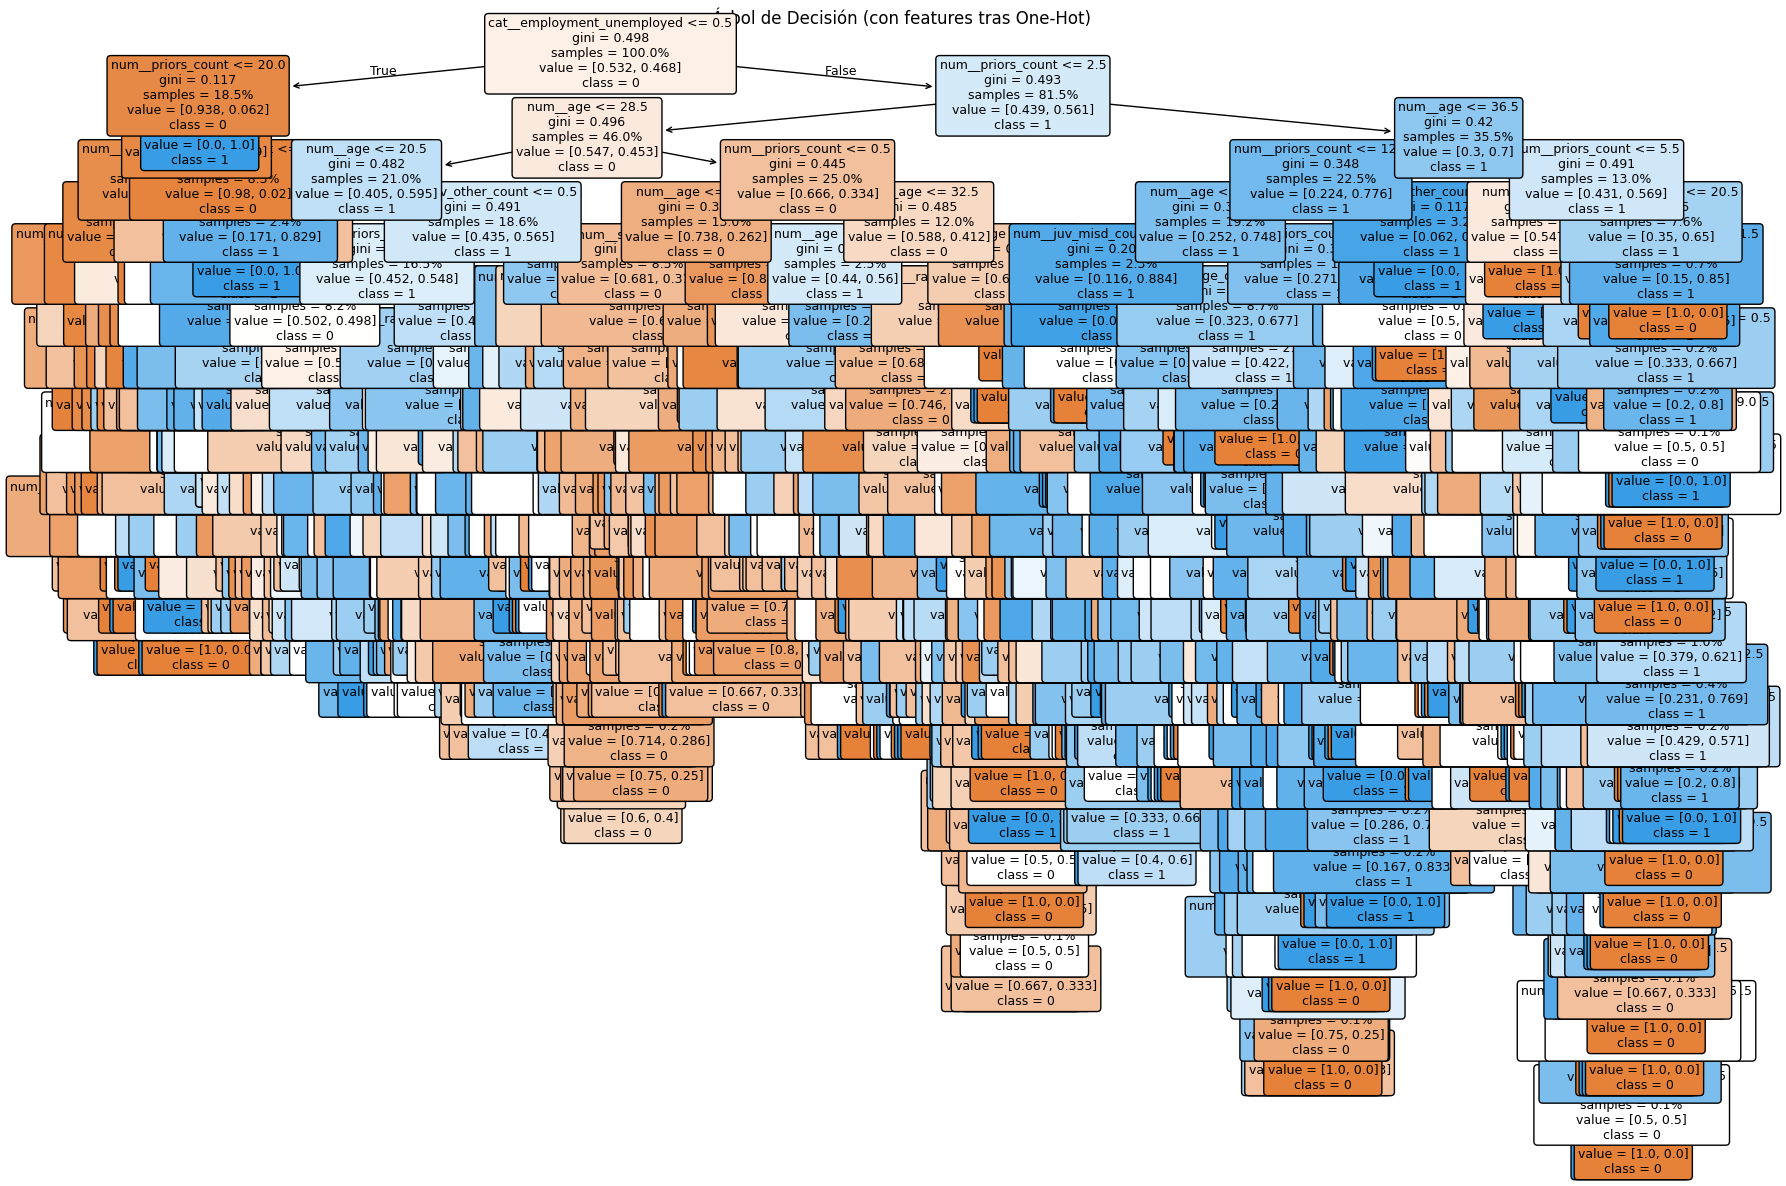
\includegraphics[width=\linewidth]{figures/decision_tree_baseline.png}
    \caption{Árbol baseline.}
  \end{subfigure}\hfill
  \begin{subfigure}[t]{0.48\linewidth}
    \centering
    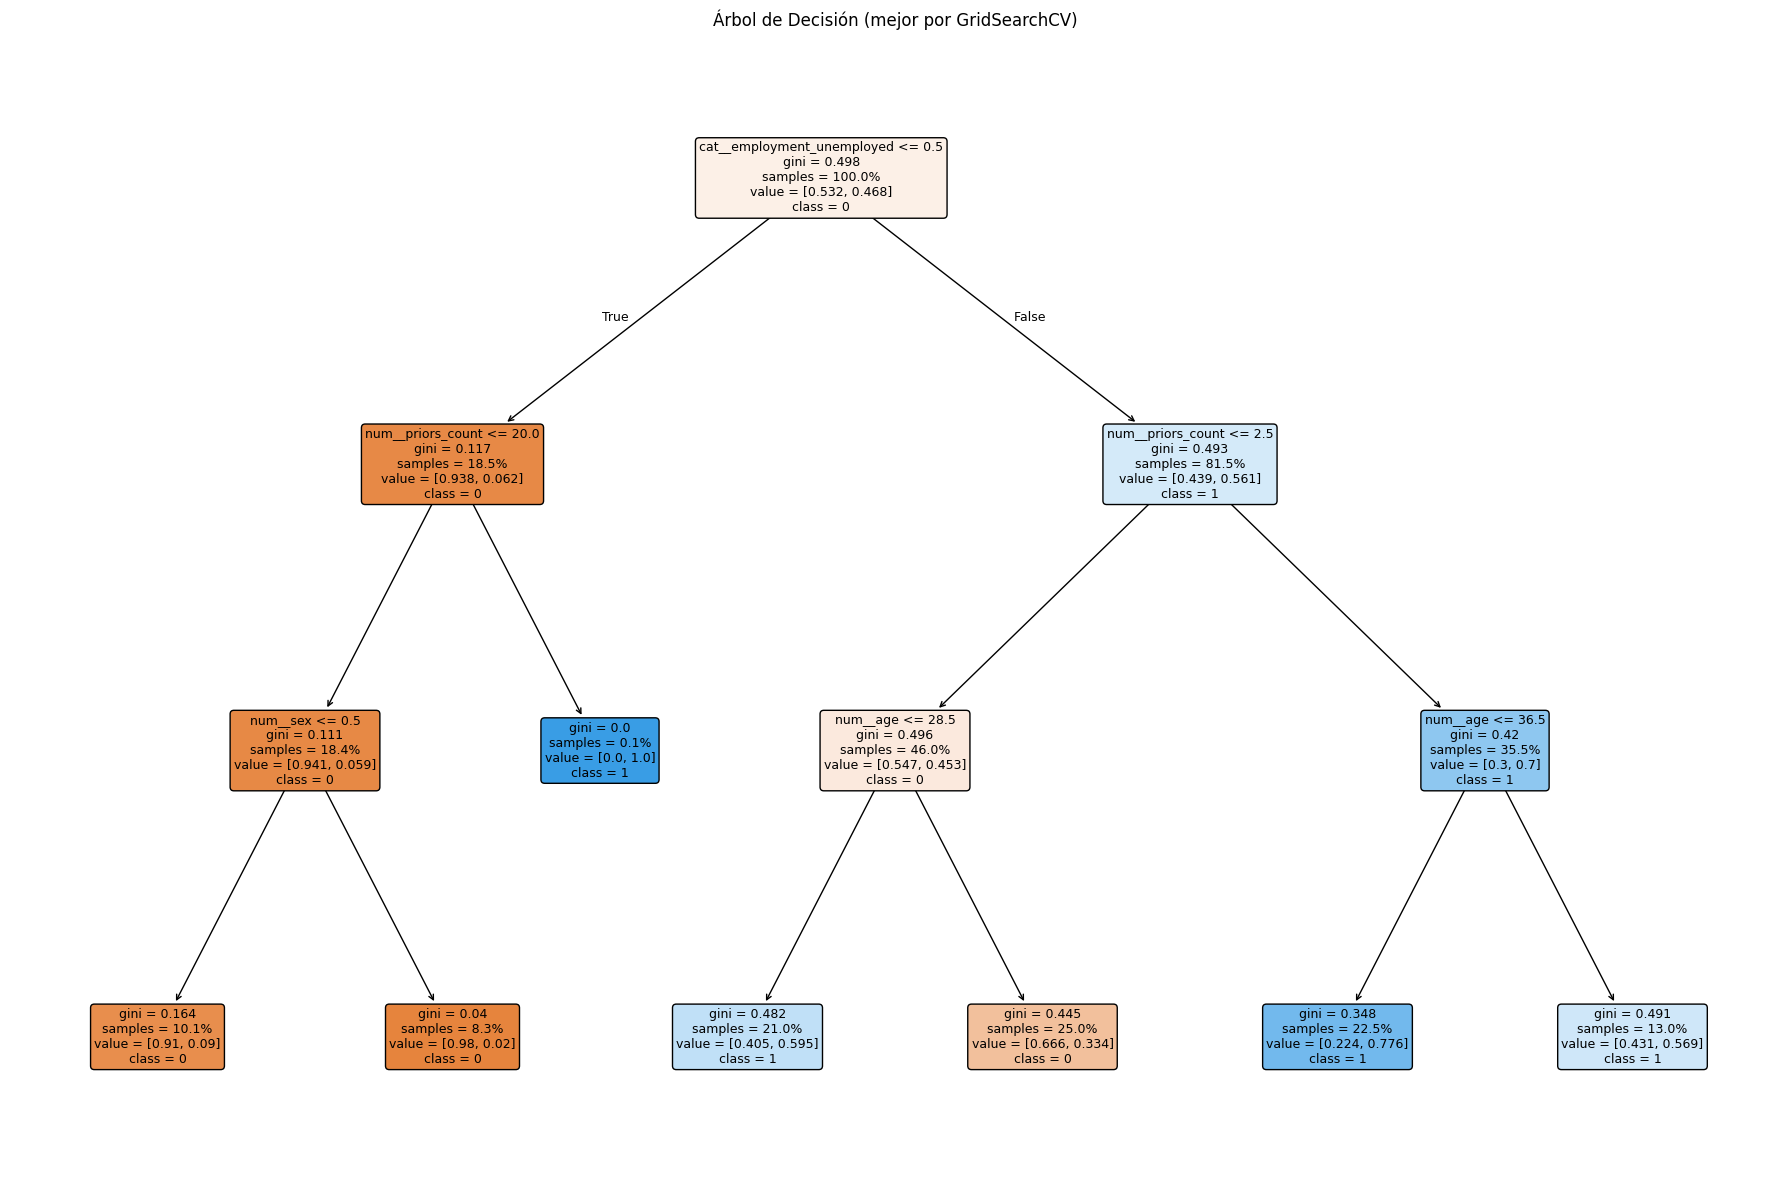
\includegraphics[width=\linewidth]{figures/decision_tree_tuned.png}
    \caption{Árbol ajustado (GridSearch).}
  \end{subfigure}
  \caption{Comparativa visual de los árboles baseline y ajustado. El modelo ajustado presenta menor profundidad y una jerarquía de decisiones más estable.}
\end{figure}

\subsection{Estudio de linealidad y unificación de variables}

El análisis de correlaciones mostró valores moderados (entre $-0.2$ y $+0.3$), lo que indica la \textbf{ausencia de multicolinealidad fuerte} y sugiere que las variables son en general independientes. Esto permite aplicar tanto modelos logísticos como aditivos sin comprometer la estabilidad de los coeficientes.

Con el objetivo de profundizar en las relaciones entre las variables numéricas y la probabilidad de reincidencia, se realizó un \textbf{estudio de linealidad} para observar el comportamiento individual de cada predictor frente a la variable objetivo. La \autoref{fig:linearidad} muestra cómo, aunque algunas relaciones son aproximadamente proporcionales, otras presentan patrones no lineales que justifican el uso de un modelo aditivo (GAM).

\begin{itemize}
  \item \textbf{age}: relación inversa clara con la reincidencia; a menor edad, mayor probabilidad de reincidencia.
  \item \textbf{priors\_count}: efecto creciente con tendencia a saturarse a partir de $\sim$20 antecedentes.
  \item \textbf{juv\_fel\_count}: leve relación positiva, aunque con dispersión limitada.
  \item \textbf{juv\_misd\_count}: comportamiento no lineal e irregular, reflejando un posible efecto umbral.
  \item \textbf{juv\_other\_count}: correlación débil y poco estructurada con el objetivo.
\end{itemize}

Estos resultados confirman que \textbf{la edad y los antecedentes previos} son los principales determinantes de la reincidencia, pero su relación no es estrictamente lineal. Por ello, además del modelo logístico, se incorporó un modelo aditivo capaz de capturar estas transiciones suaves de riesgo.

\begin{figure}[h]
  \centering
  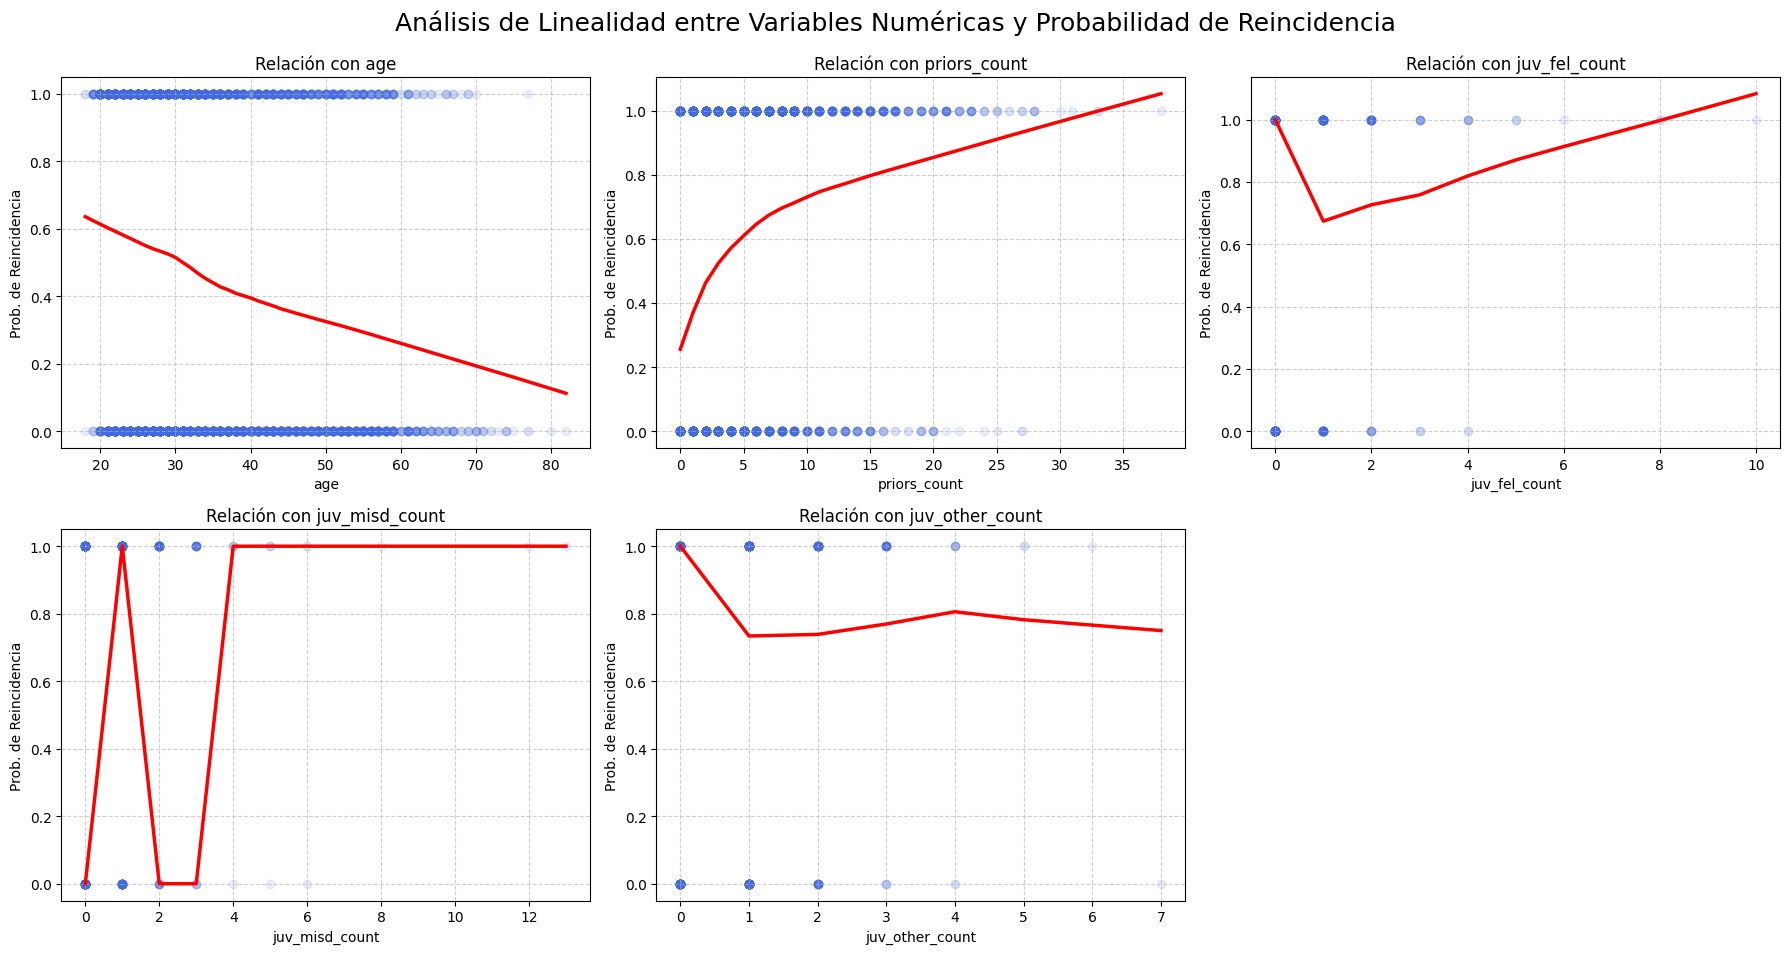
\includegraphics[width=\linewidth]{figures/linearidad_variables.png}
  \caption{Análisis de linealidad entre variables numéricas y probabilidad de reincidencia. 
  Las líneas rojas representan la tendencia media (efecto parcial) y los puntos azules los valores observados. 
  Se observa un patrón no lineal claro en \texttt{priors\_count} y \texttt{age}, lo que motiva el uso del modelo aditivo (GAM).}
  \label{fig:linearidad}
\end{figure}

Complementariamente, se analizó la \textbf{tasa media de reincidencia para variables categóricas y binarias}, con el fin de comprender mejor el comportamiento de los grupos sociales y judiciales presentes en el conjunto de datos.  
Como muestra la \autoref{fig:tasa_categoricas}, los individuos desempleados presentan una tasa de reincidencia notablemente superior (0.56) frente a los empleados (0.06), mientras que las diferencias por sexo y tipo de cargo son más moderadas pero consistentes.  
Asimismo, el grupo \texttt{is\_AfricanAmerican\_vs\_Caucasian} muestra una ligera mayor tasa de reincidencia en la población afroamericana (0.52 frente a 0.40), coherente con los patrones descritos en la literatura previa sobre sesgos y factores socioeconómicos.


Estos patrones refuerzan la idea de que los factores socioeconómicos y demográficos condicionan la probabilidad de reincidencia, y justifican la unificación de variables redundantes para facilitar la interpretación de los modelos explicativos.

Asimismo, se detectaron \textbf{variables redundantes} derivadas de la codificación One-HotEncoder, como
race\_Caucasian / race\_African-American,
c\_charge\_degree\_F / c\_charge\_degree\_M, y
sex\_Male / sex\_Female. 
Estas variables fueron unificadas mediante una función de preprocesado que las combinó en comparaciones binarias más interpretables: is\_AfricanAmerican\_vs\_Caucasian,
is\_Felony\_vs\_Misdemeanor y
is\_Male\_vs\_Female, reduciendo redundancias y mejorando la estabilidad del modelo logístico.

\begin{figure}[h]
  \centering
  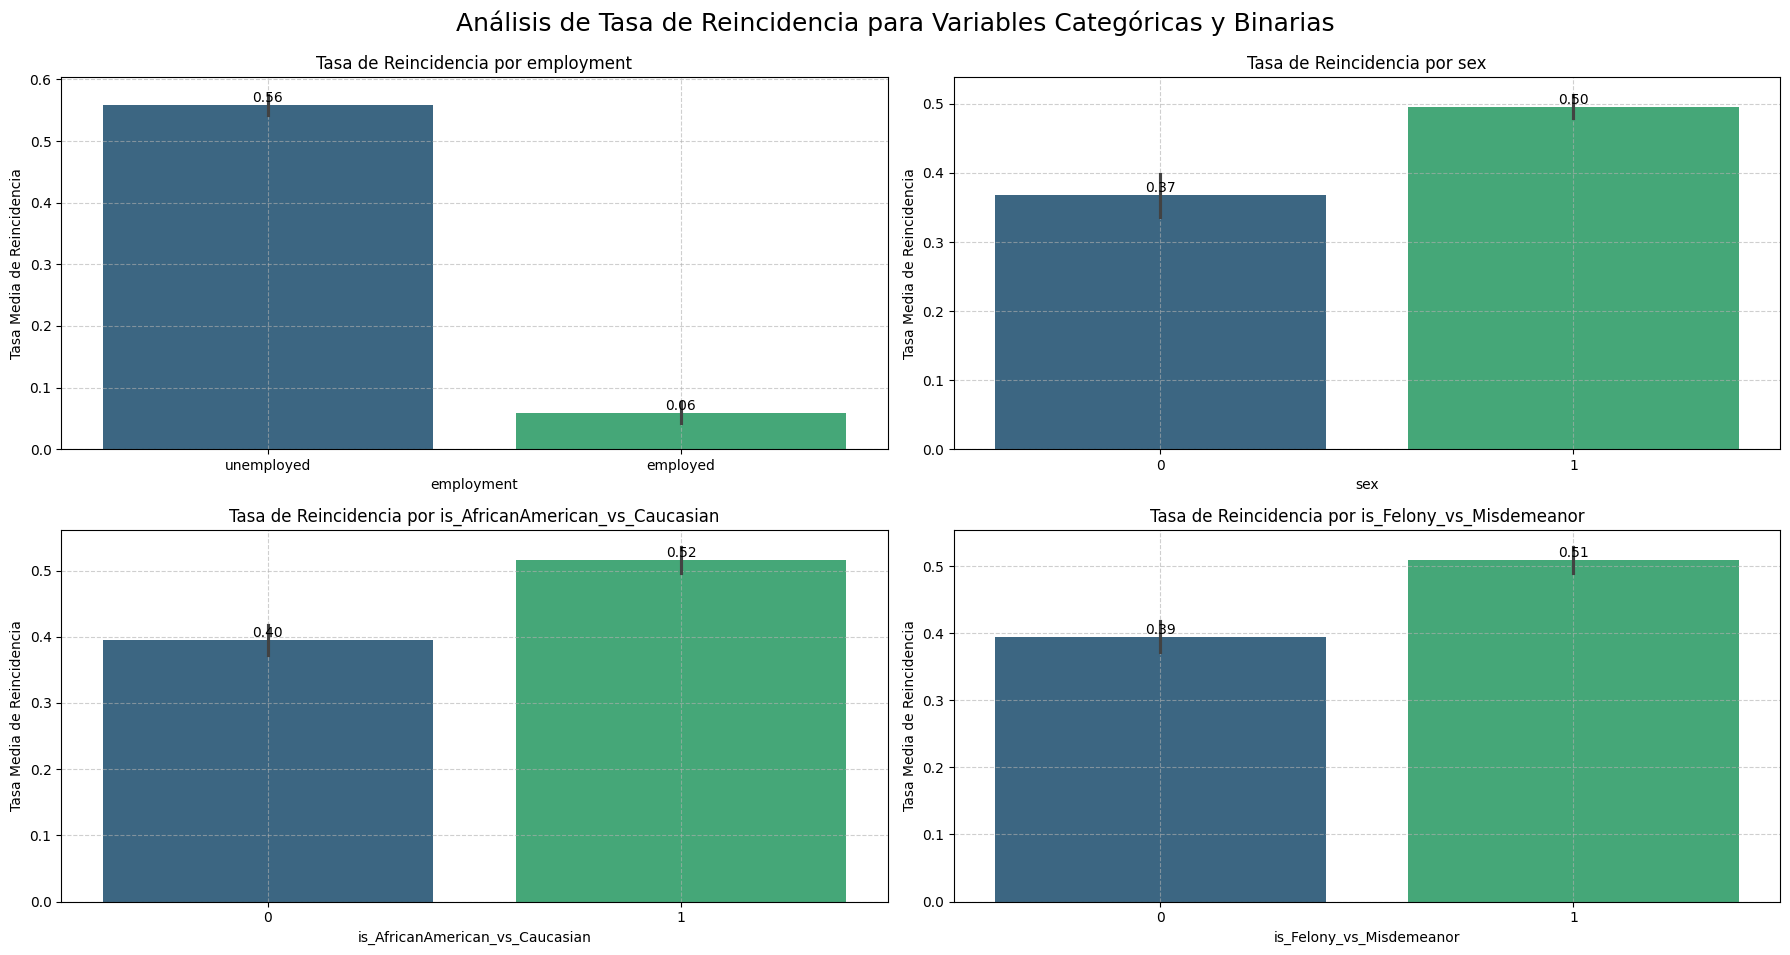
\includegraphics[width=\linewidth]{figures/tasa_categoricas.png}
  \caption{Tasa media de reincidencia por variables categóricas y binarias. 
  Se observa una diferencia marcada por empleo, con tasas de reincidencia más altas entre personas desempleadas. 
  Las diferencias por sexo, raza y tipo de cargo son más suaves pero mantienen coherencia en la dirección del efecto.}
  \label{fig:tasa_categoricas}
\end{figure}


\subsection{Modelo logístico}

El modelo \textbf{logístico} actúa como una referencia intermedia entre el árbol y el GAM. Ofrece una lectura directa de los coeficientes (signo y magnitud) y permite cuantificar el impacto de cada variable sobre la probabilidad de reincidencia. En validación se observó una \textbf{Accuracy (valid) $\approx$ 0.70} y un comportamiento equilibrado entre clases. Los coeficientes positivos se asocian a \texttt{priors\_count} y a la condición de desempleo, mientras que los negativos a \texttt{age} y a la categoría de empleo estable, que funcionan como factores protectores.

El ajuste mediante \texttt{GridSearchCV} exploró distintos valores de regularización \texttt{C}, penalización \texttt{L2} y solvers, identificando un modelo estable y bien calibrado. Aunque su estructura lineal limita la capacidad de capturar interacciones o efectos no lineales, el modelo destaca por su \textbf{claridad interpretativa y consistencia estadística}, manteniendo una brecha reducida entre entrenamiento y validación.

\subsection{Modelo aditivo (GAM / EBM)}

El \textbf{GAM/EBM}, implementado mediante \texttt{ExplainableBoostingClassifier}, combina la flexibilidad de los modelos no lineales con la interpretabilidad de los modelos aditivos. Cada predictor se modela mediante una función de forma libre y el resultado se obtiene como la suma de los efectos individuales. En validación, el EBM alcanzó una \textbf{Accuracy (valid) $\approx$ 0.72}, mejorando tanto al árbol ajustado como al modelo logístico.

Las curvas globales del EBM muestran un patrón coherente con el análisis exploratorio: el riesgo de reincidencia aumenta con el número de antecedentes y disminuye con la edad, de forma no lineal. La versión con un número limitado de interacciones (\texttt{interactions = 5}) aportó una ligera mejora en precisión sin comprometer la explicabilidad, destacando combinaciones intuitivas como edad y antecedentes.

En conjunto, el modelo aditivo se consolidó como el \textbf{más equilibrado} del estudio: logró la mejor generalización, explicó correctamente las tendencias observadas y mantuvo una estructura fácilmente interpretable tanto a nivel global (efectos parciales) como local (contribuciones por individuo).

\paragraph{Lectura conjunta.}
El \textbf{árbol ajustado} supera al baseline y estabiliza las reglas de decisión; el \textbf{modelo logístico} aporta claridad interpretativa y resultados consistentes; y el \textbf{GAM/EBM} logra el mejor equilibrio entre rendimiento y explicabilidad. La progresión entre los tres modelos refleja cómo un incremento gradual en complejidad estructural permite capturar mejor los patrones del fenómeno sin perder transparencia ni robustez.
